\documentclass[]{article}
\usepackage{lmodern}
\usepackage{amssymb,amsmath}
\usepackage{ifxetex,ifluatex}
\usepackage{fixltx2e} % provides \textsubscript
\ifnum 0\ifxetex 1\fi\ifluatex 1\fi=0 % if pdftex
  \usepackage[T1]{fontenc}
  \usepackage[utf8]{inputenc}
\else % if luatex or xelatex
  \ifxetex
    \usepackage{mathspec}
  \else
    \usepackage{fontspec}
  \fi
  \defaultfontfeatures{Ligatures=TeX,Scale=MatchLowercase}
\fi
% use upquote if available, for straight quotes in verbatim environments
\IfFileExists{upquote.sty}{\usepackage{upquote}}{}
% use microtype if available
\IfFileExists{microtype.sty}{%
\usepackage{microtype}
\UseMicrotypeSet[protrusion]{basicmath} % disable protrusion for tt fonts
}{}
\usepackage[margin=1in]{geometry}
\usepackage{hyperref}
\hypersetup{unicode=true,
            pdftitle={Introduction to R and RStudio},
            pdfborder={0 0 0},
            breaklinks=true}
\urlstyle{same}  % don't use monospace font for urls
\usepackage{color}
\usepackage{fancyvrb}
\newcommand{\VerbBar}{|}
\newcommand{\VERB}{\Verb[commandchars=\\\{\}]}
\DefineVerbatimEnvironment{Highlighting}{Verbatim}{commandchars=\\\{\}}
% Add ',fontsize=\small' for more characters per line
\usepackage{framed}
\definecolor{shadecolor}{RGB}{248,248,248}
\newenvironment{Shaded}{\begin{snugshade}}{\end{snugshade}}
\newcommand{\KeywordTok}[1]{\textcolor[rgb]{0.13,0.29,0.53}{\textbf{#1}}}
\newcommand{\DataTypeTok}[1]{\textcolor[rgb]{0.13,0.29,0.53}{#1}}
\newcommand{\DecValTok}[1]{\textcolor[rgb]{0.00,0.00,0.81}{#1}}
\newcommand{\BaseNTok}[1]{\textcolor[rgb]{0.00,0.00,0.81}{#1}}
\newcommand{\FloatTok}[1]{\textcolor[rgb]{0.00,0.00,0.81}{#1}}
\newcommand{\ConstantTok}[1]{\textcolor[rgb]{0.00,0.00,0.00}{#1}}
\newcommand{\CharTok}[1]{\textcolor[rgb]{0.31,0.60,0.02}{#1}}
\newcommand{\SpecialCharTok}[1]{\textcolor[rgb]{0.00,0.00,0.00}{#1}}
\newcommand{\StringTok}[1]{\textcolor[rgb]{0.31,0.60,0.02}{#1}}
\newcommand{\VerbatimStringTok}[1]{\textcolor[rgb]{0.31,0.60,0.02}{#1}}
\newcommand{\SpecialStringTok}[1]{\textcolor[rgb]{0.31,0.60,0.02}{#1}}
\newcommand{\ImportTok}[1]{#1}
\newcommand{\CommentTok}[1]{\textcolor[rgb]{0.56,0.35,0.01}{\textit{#1}}}
\newcommand{\DocumentationTok}[1]{\textcolor[rgb]{0.56,0.35,0.01}{\textbf{\textit{#1}}}}
\newcommand{\AnnotationTok}[1]{\textcolor[rgb]{0.56,0.35,0.01}{\textbf{\textit{#1}}}}
\newcommand{\CommentVarTok}[1]{\textcolor[rgb]{0.56,0.35,0.01}{\textbf{\textit{#1}}}}
\newcommand{\OtherTok}[1]{\textcolor[rgb]{0.56,0.35,0.01}{#1}}
\newcommand{\FunctionTok}[1]{\textcolor[rgb]{0.00,0.00,0.00}{#1}}
\newcommand{\VariableTok}[1]{\textcolor[rgb]{0.00,0.00,0.00}{#1}}
\newcommand{\ControlFlowTok}[1]{\textcolor[rgb]{0.13,0.29,0.53}{\textbf{#1}}}
\newcommand{\OperatorTok}[1]{\textcolor[rgb]{0.81,0.36,0.00}{\textbf{#1}}}
\newcommand{\BuiltInTok}[1]{#1}
\newcommand{\ExtensionTok}[1]{#1}
\newcommand{\PreprocessorTok}[1]{\textcolor[rgb]{0.56,0.35,0.01}{\textit{#1}}}
\newcommand{\AttributeTok}[1]{\textcolor[rgb]{0.77,0.63,0.00}{#1}}
\newcommand{\RegionMarkerTok}[1]{#1}
\newcommand{\InformationTok}[1]{\textcolor[rgb]{0.56,0.35,0.01}{\textbf{\textit{#1}}}}
\newcommand{\WarningTok}[1]{\textcolor[rgb]{0.56,0.35,0.01}{\textbf{\textit{#1}}}}
\newcommand{\AlertTok}[1]{\textcolor[rgb]{0.94,0.16,0.16}{#1}}
\newcommand{\ErrorTok}[1]{\textcolor[rgb]{0.64,0.00,0.00}{\textbf{#1}}}
\newcommand{\NormalTok}[1]{#1}
\usepackage{graphicx,grffile}
\makeatletter
\def\maxwidth{\ifdim\Gin@nat@width>\linewidth\linewidth\else\Gin@nat@width\fi}
\def\maxheight{\ifdim\Gin@nat@height>\textheight\textheight\else\Gin@nat@height\fi}
\makeatother
% Scale images if necessary, so that they will not overflow the page
% margins by default, and it is still possible to overwrite the defaults
% using explicit options in \includegraphics[width, height, ...]{}
\setkeys{Gin}{width=\maxwidth,height=\maxheight,keepaspectratio}
\IfFileExists{parskip.sty}{%
\usepackage{parskip}
}{% else
\setlength{\parindent}{0pt}
\setlength{\parskip}{6pt plus 2pt minus 1pt}
}
\setlength{\emergencystretch}{3em}  % prevent overfull lines
\providecommand{\tightlist}{%
  \setlength{\itemsep}{0pt}\setlength{\parskip}{0pt}}
\setcounter{secnumdepth}{0}
% Redefines (sub)paragraphs to behave more like sections
\ifx\paragraph\undefined\else
\let\oldparagraph\paragraph
\renewcommand{\paragraph}[1]{\oldparagraph{#1}\mbox{}}
\fi
\ifx\subparagraph\undefined\else
\let\oldsubparagraph\subparagraph
\renewcommand{\subparagraph}[1]{\oldsubparagraph{#1}\mbox{}}
\fi

%%% Use protect on footnotes to avoid problems with footnotes in titles
\let\rmarkdownfootnote\footnote%
\def\footnote{\protect\rmarkdownfootnote}

%%% Change title format to be more compact
\usepackage{titling}

% Create subtitle command for use in maketitle
\newcommand{\subtitle}[1]{
  \posttitle{
    \begin{center}\large#1\end{center}
    }
}

\setlength{\droptitle}{-2em}

  \title{Introduction to R and RStudio}
    \pretitle{\vspace{\droptitle}\centering\huge}
  \posttitle{\par}
    \author{}
    \preauthor{}\postauthor{}
    \date{}
    \predate{}\postdate{}
  

\begin{document}
\maketitle

The goal of this lab is to introduce you to R and RStudio, which you'll
be using throughout the course both to learn the statistical concepts
discussed in the texbook and also to analyze real data and come to
informed conclusions. To straighten out which is which: R is the name of
the programming language itself and RStudio is a convenient interface.

As the labs progress, you are encouraged to explore beyond what the labs
dictate; a willingness to experiment will make you a much better
programmer. Before we get to that stage, however, you need to build some
basic fluency in R. Today we begin with the fundamental building blocks
of R and RStudio: the interface, reading in data, and basic commands.

\begin{figure}
\centering
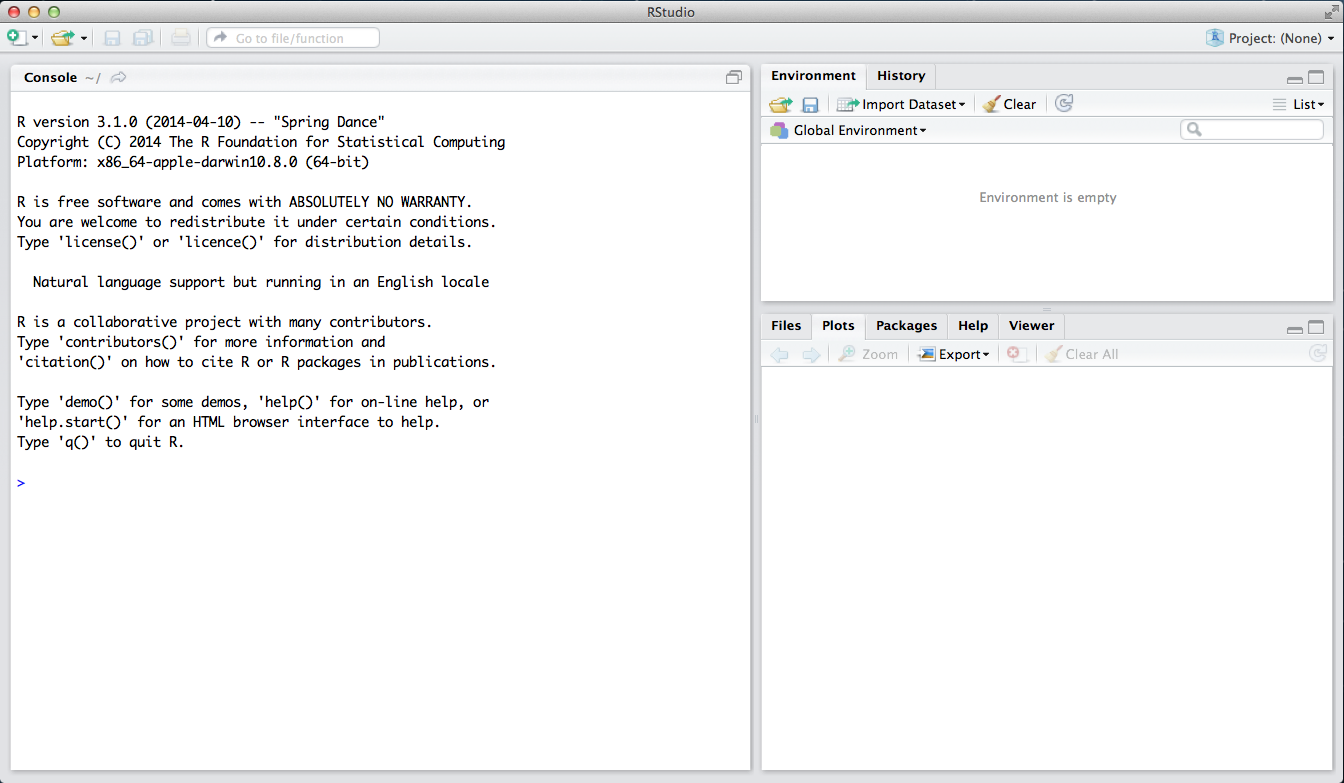
\includegraphics{more/rInterface2014.png}
\caption{rinterface}
\end{figure}

The panel in the upper right contains your \emph{workspace} as well as a
history of the commands that you've previously entered. Any plots that
you generate will show up in the panel in the lower right corner.

The panel on the left is where the action happens. It's called the
\emph{console}. Everytime you launch RStudio, it will have the same text
at the top of the console telling you the version of R that you're
running. Below that information is the \emph{prompt}. As its name
suggests, this prompt is really a request, a request for a command.
Initially, interacting with R is all about typing commands and
interpreting the output. These commands and their syntax have evolved
over decades (literally) and now provide what many users feel is a
fairly natural way to access data and organize, describe, and invoke
statistical computations.

To get you started, enter the following command at the R prompt
(i.e.~right after \texttt{\textgreater{}} on the console). You can
either type it in manually or copy and paste it from this document.

\begin{verbatim}
## Installing package into 'C:/Users/Chandini/Documents/R/win-library/3.5'
## (as 'lib' is unspecified)
\end{verbatim}

\begin{verbatim}
## package 'tinytex' successfully unpacked and MD5 sums checked
## 
## The downloaded binary packages are in
##  C:\Users\Chandini\AppData\Local\Temp\RtmpQdF7ol\downloaded_packages
\end{verbatim}

\begin{verbatim}
## Warning: package 'tinytex' was built under R version 3.5.2
\end{verbatim}

\begin{Shaded}
\begin{Highlighting}[]
\KeywordTok{source}\NormalTok{(}\StringTok{"more/arbuthnot.R"}\NormalTok{)}
\end{Highlighting}
\end{Shaded}

This command instructs R to access the OpenIntro website and fetch some
data: the Arbuthnot baptism counts for boys and girls. You should see
that the workspace area in the upper righthand corner of the RStudio
window now lists a data set called \texttt{arbuthnot} that has 82
observations on 3 variables. As you interact with R, you will create a
series of objects. Sometimes you load them as we have done here, and
sometimes you create them yourself as the byproduct of a computation or
some analysis you have performed. Note that because you are accessing
data from the web, this command (and the entire assignment) will work in
a computer lab, in the library, or in your dorm room; anywhere you have
access to the Internet.

\subsection{The Data: Dr.~Arbuthnot's Baptism
Records}\label{the-data-dr.arbuthnots-baptism-records}

The Arbuthnot data set refers to Dr.~John Arbuthnot, an 18th century
physician, writer, and mathematician. He was interested in the ratio of
newborn boys to newborn girls, so he gathered the baptism records for
children born in London for every year from 1629 to 1710. We can take a
look at the data by typing its name into the console.

\begin{Shaded}
\begin{Highlighting}[]
\NormalTok{arbuthnot}
\end{Highlighting}
\end{Shaded}

\begin{verbatim}
##    year boys girls
## 1  1629 5218  4683
## 2  1630 4858  4457
## 3  1631 4422  4102
## 4  1632 4994  4590
## 5  1633 5158  4839
## 6  1634 5035  4820
## 7  1635 5106  4928
## 8  1636 4917  4605
## 9  1637 4703  4457
## 10 1638 5359  4952
## 11 1639 5366  4784
## 12 1640 5518  5332
## 13 1641 5470  5200
## 14 1642 5460  4910
## 15 1643 4793  4617
## 16 1644 4107  3997
## 17 1645 4047  3919
## 18 1646 3768  3395
## 19 1647 3796  3536
## 20 1648 3363  3181
## 21 1649 3079  2746
## 22 1650 2890  2722
## 23 1651 3231  2840
## 24 1652 3220  2908
## 25 1653 3196  2959
## 26 1654 3441  3179
## 27 1655 3655  3349
## 28 1656 3668  3382
## 29 1657 3396  3289
## 30 1658 3157  3013
## 31 1659 3209  2781
## 32 1660 3724  3247
## 33 1661 4748  4107
## 34 1662 5216  4803
## 35 1663 5411  4881
## 36 1664 6041  5681
## 37 1665 5114  4858
## 38 1666 4678  4319
## 39 1667 5616  5322
## 40 1668 6073  5560
## 41 1669 6506  5829
## 42 1670 6278  5719
## 43 1671 6449  6061
## 44 1672 6443  6120
## 45 1673 6073  5822
## 46 1674 6113  5738
## 47 1675 6058  5717
## 48 1676 6552  5847
## 49 1677 6423  6203
## 50 1678 6568  6033
## 51 1679 6247  6041
## 52 1680 6548  6299
## 53 1681 6822  6533
## 54 1682 6909  6744
## 55 1683 7577  7158
## 56 1684 7575  7127
## 57 1685 7484  7246
## 58 1686 7575  7119
## 59 1687 7737  7214
## 60 1688 7487  7101
## 61 1689 7604  7167
## 62 1690 7909  7302
## 63 1691 7662  7392
## 64 1692 7602  7316
## 65 1693 7676  7483
## 66 1694 6985  6647
## 67 1695 7263  6713
## 68 1696 7632  7229
## 69 1697 8062  7767
## 70 1698 8426  7626
## 71 1699 7911  7452
## 72 1700 7578  7061
## 73 1701 8102  7514
## 74 1702 8031  7656
## 75 1703 7765  7683
## 76 1704 6113  5738
## 77 1705 8366  7779
## 78 1706 7952  7417
## 79 1707 8379  7687
## 80 1708 8239  7623
## 81 1709 7840  7380
## 82 1710 7640  7288
\end{verbatim}

What you should see are four columns of numbers, each row representing a
different year: the first entry in each row is simply the row number (an
index we can use to access the data from individual years if we want),
the second is the year, and the third and fourth are the numbers of boys
and girls baptized that year, respectively. Use the scrollbar on the
right side of the console window to examine the complete data set.

Note that the row numbers in the first column are not part of
Arbuthnot's data. R adds them as part of its printout to help you make
visual comparisons. You can think of them as the index that you see on
the left side of a spreadsheet. In fact, the comparison to a spreadsheet
will generally be helpful. R has stored Arbuthnot's data in a kind of
spreadsheet or table called a \emph{data frame}.

You can see the dimensions of this data frame by typing:

\begin{Shaded}
\begin{Highlighting}[]
\KeywordTok{dim}\NormalTok{(arbuthnot)}
\end{Highlighting}
\end{Shaded}

\begin{verbatim}
## [1] 82  3
\end{verbatim}

This command should output \texttt{{[}1{]}\ 82\ 3}, indicating that
there are 82 rows and 3 columns (we'll get to what the \texttt{{[}1{]}}
means in a bit), just as it says next to the object in your workspace.
You can see the names of these columns (or variables) by typing:

\begin{Shaded}
\begin{Highlighting}[]
\KeywordTok{names}\NormalTok{(arbuthnot)}
\end{Highlighting}
\end{Shaded}

\begin{verbatim}
## [1] "year"  "boys"  "girls"
\end{verbatim}

You should see that the data frame contains the columns \texttt{year},
\texttt{boys}, and \texttt{girls}. At this point, you might notice that
many of the commands in R look a lot like functions from math class;
that is, invoking R commands means supplying a function with some number
of arguments. The \texttt{dim} and \texttt{names} commands, for example,
each took a single argument, the name of a data frame.

One advantage of RStudio is that it comes with a built-in data viewer.
Click on the name \texttt{arbuthnot} in the \emph{Environment} pane
(upper right window) that lists the objects in your workspace. This will
bring up an alternative display of the data set in the \emph{Data
Viewer} (upper left window). You can close the data viewer by clicking
on the \emph{x} in the upper lefthand corner.

\subsection{Some Exploration}\label{some-exploration}

Let's start to examine the data a little more closely. We can access the
data in a single column of a data frame separately using a command like

\begin{Shaded}
\begin{Highlighting}[]
\NormalTok{arbuthnot}\OperatorTok{$}\NormalTok{boys}
\end{Highlighting}
\end{Shaded}

\begin{verbatim}
##  [1] 5218 4858 4422 4994 5158 5035 5106 4917 4703 5359 5366 5518 5470 5460
## [15] 4793 4107 4047 3768 3796 3363 3079 2890 3231 3220 3196 3441 3655 3668
## [29] 3396 3157 3209 3724 4748 5216 5411 6041 5114 4678 5616 6073 6506 6278
## [43] 6449 6443 6073 6113 6058 6552 6423 6568 6247 6548 6822 6909 7577 7575
## [57] 7484 7575 7737 7487 7604 7909 7662 7602 7676 6985 7263 7632 8062 8426
## [71] 7911 7578 8102 8031 7765 6113 8366 7952 8379 8239 7840 7640
\end{verbatim}

This command will only show the number of boys baptized each year.

\begin{enumerate}
\def\labelenumi{\arabic{enumi}.}
\tightlist
\item
  What command would you use to extract just the counts of girls
  baptized? Try it! \textbf{Answer: arbuthnot\$girls}
\end{enumerate}

Notice that the way R has printed these data is different. When we
looked at the complete data frame, we saw 82 rows, one on each line of
the display. These data are no longer structured in a table with other
variables, so they are displayed one right after another. Objects that
print out in this way are called \emph{vectors}; they represent a set of
numbers. R has added numbers in {[}brackets{]} along the left side of
the printout to indicate locations within the vector. For example,
\texttt{5218} follows \texttt{{[}1{]}}, indicating that \texttt{5218} is
the first entry in the vector. And if \texttt{{[}43{]}} starts a line,
then that would mean the first number on that line would represent the
43rd entry in the vector.

R has some powerful functions for making graphics. We can create a
simple plot of the number of girls baptized per year with the command

\begin{Shaded}
\begin{Highlighting}[]
\KeywordTok{plot}\NormalTok{(}\DataTypeTok{x =}\NormalTok{ arbuthnot}\OperatorTok{$}\NormalTok{year, }\DataTypeTok{y =}\NormalTok{ arbuthnot}\OperatorTok{$}\NormalTok{girls)}
\end{Highlighting}
\end{Shaded}

\includegraphics{Santosh-intro_to_r_files/figure-latex/plot-girls-vs-year-1.pdf}

By default, R creates a scatterplot with each x,y pair indicated by an
open circle. The plot itself should appear under the \emph{Plots} tab of
the lower right panel of RStudio. Notice that the command above again
looks like a function, this time with two arguments separated by a
comma. The first argument in the plot function specifies the variable
for the x-axis and the second for the y-axis. If we wanted to connect
the data points with lines, we could add a third argument, the letter
\texttt{l} for \textbf{l}ine.

\begin{Shaded}
\begin{Highlighting}[]
\KeywordTok{plot}\NormalTok{(}\DataTypeTok{x =}\NormalTok{ arbuthnot}\OperatorTok{$}\NormalTok{year, }\DataTypeTok{y =}\NormalTok{ arbuthnot}\OperatorTok{$}\NormalTok{girls, }\DataTypeTok{type =} \StringTok{"l"}\NormalTok{)}
\end{Highlighting}
\end{Shaded}

\includegraphics{Santosh-intro_to_r_files/figure-latex/plot-girls-vs-year-line-1.pdf}

You might wonder how you are supposed to know that it was possible to
add that third argument. Thankfully, R documents all of its functions
extensively. To read what a function does and learn the arguments that
are available to you, just type in a question mark followed by the name
of the function that you're interested in. Try the following.

\begin{Shaded}
\begin{Highlighting}[]
\NormalTok{?plot}
\end{Highlighting}
\end{Shaded}

\begin{verbatim}
## starting httpd help server ... done
\end{verbatim}

Notice that the help file replaces the plot in the lower right panel.
You can toggle between plots and help files using the tabs at the top of
that panel.

\begin{enumerate}
\def\labelenumi{\arabic{enumi}.}
\setcounter{enumi}{1}
\tightlist
\item
  Is there an apparent trend in the number of girls baptized over the
  years?\\
  How would you describe it? \textbf{Answer: There was decline in number
  of baptized girls from 1640 to 1660, but rose again from 1660 hitting
  a max around 1700's}
\end{enumerate}

Now, suppose we want to plot the total number of baptisms. To compute
this, we could use the fact that R is really just a big calculator. We
can type in mathematical expressions like

\begin{Shaded}
\begin{Highlighting}[]
\DecValTok{5218} \OperatorTok{+}\StringTok{ }\DecValTok{4683}
\end{Highlighting}
\end{Shaded}

\begin{verbatim}
## [1] 9901
\end{verbatim}

to see the total number of baptisms in 1629. We could repeat this once
for each year, but there is a faster way. If we add the vector for
baptisms for boys and girls, R will compute all sums simultaneously.

\begin{Shaded}
\begin{Highlighting}[]
\NormalTok{arbuthnot}\OperatorTok{$}\NormalTok{boys }\OperatorTok{+}\StringTok{ }\NormalTok{arbuthnot}\OperatorTok{$}\NormalTok{girls}
\end{Highlighting}
\end{Shaded}

\begin{verbatim}
##  [1]  9901  9315  8524  9584  9997  9855 10034  9522  9160 10311 10150
## [12] 10850 10670 10370  9410  8104  7966  7163  7332  6544  5825  5612
## [23]  6071  6128  6155  6620  7004  7050  6685  6170  5990  6971  8855
## [34] 10019 10292 11722  9972  8997 10938 11633 12335 11997 12510 12563
## [45] 11895 11851 11775 12399 12626 12601 12288 12847 13355 13653 14735
## [56] 14702 14730 14694 14951 14588 14771 15211 15054 14918 15159 13632
## [67] 13976 14861 15829 16052 15363 14639 15616 15687 15448 11851 16145
## [78] 15369 16066 15862 15220 14928
\end{verbatim}

What you will see are 82 numbers (in that packed display, because we
aren't looking at a data frame here), each one representing the sum
we're after. Take a look at a few of them and verify that they are
right. Therefore, we can make a plot of the total number of baptisms per
year with the command

\begin{Shaded}
\begin{Highlighting}[]
\KeywordTok{plot}\NormalTok{(arbuthnot}\OperatorTok{$}\NormalTok{year, arbuthnot}\OperatorTok{$}\NormalTok{boys }\OperatorTok{+}\StringTok{ }\NormalTok{arbuthnot}\OperatorTok{$}\NormalTok{girls, }\DataTypeTok{type =} \StringTok{"l"}\NormalTok{)}
\end{Highlighting}
\end{Shaded}

\includegraphics{Santosh-intro_to_r_files/figure-latex/plot-total-vs-year-1.pdf}

This time, note that we left out the names of the first two arguments.
We can do this because the help file shows that the default for
\texttt{plot} is for the first argument to be the x-variable and the
second argument to be the y-variable.

Similarly to how we computed the proportion of boys, we can compute the
ratio of the number of boys to the number of girls baptized in 1629 with

\begin{Shaded}
\begin{Highlighting}[]
\DecValTok{5218} \OperatorTok{/}\StringTok{ }\DecValTok{4683}
\end{Highlighting}
\end{Shaded}

\begin{verbatim}
## [1] 1.114243
\end{verbatim}

or we can act on the complete vectors with the expression

\begin{Shaded}
\begin{Highlighting}[]
\NormalTok{arbuthnot}\OperatorTok{$}\NormalTok{boys }\OperatorTok{/}\StringTok{ }\NormalTok{arbuthnot}\OperatorTok{$}\NormalTok{girls}
\end{Highlighting}
\end{Shaded}

\begin{verbatim}
##  [1] 1.114243 1.089971 1.078011 1.088017 1.065923 1.044606 1.036120
##  [8] 1.067752 1.055194 1.082189 1.121656 1.034884 1.051923 1.112016
## [15] 1.038120 1.027521 1.032661 1.109867 1.073529 1.057215 1.121267
## [22] 1.061719 1.137676 1.107290 1.080095 1.082416 1.091371 1.084565
## [29] 1.032533 1.047793 1.153901 1.146905 1.156075 1.085988 1.108584
## [36] 1.063369 1.052697 1.083121 1.055242 1.092266 1.116143 1.097744
## [43] 1.064016 1.052778 1.043112 1.065354 1.059647 1.120575 1.035467
## [50] 1.088679 1.034100 1.039530 1.044237 1.024466 1.058536 1.062860
## [57] 1.032846 1.064054 1.072498 1.054359 1.060974 1.083128 1.036526
## [64] 1.039092 1.025792 1.050850 1.081931 1.055748 1.037981 1.104904
## [71] 1.061594 1.073219 1.078254 1.048981 1.010673 1.065354 1.075460
## [78] 1.072132 1.090022 1.080808 1.062331 1.048299
\end{verbatim}

The proportion of newborns that are boys

\begin{Shaded}
\begin{Highlighting}[]
\DecValTok{5218} \OperatorTok{/}\StringTok{ }\NormalTok{(}\DecValTok{5218} \OperatorTok{+}\StringTok{ }\DecValTok{4683}\NormalTok{)}
\end{Highlighting}
\end{Shaded}

\begin{verbatim}
## [1] 0.5270175
\end{verbatim}

or this may also be computed for all years simultaneously:

\begin{Shaded}
\begin{Highlighting}[]
\NormalTok{arbuthnot}\OperatorTok{$}\NormalTok{boys }\OperatorTok{/}\StringTok{ }\NormalTok{(arbuthnot}\OperatorTok{$}\NormalTok{boys }\OperatorTok{+}\StringTok{ }\NormalTok{arbuthnot}\OperatorTok{$}\NormalTok{girls)}
\end{Highlighting}
\end{Shaded}

\begin{verbatim}
##  [1] 0.5270175 0.5215244 0.5187705 0.5210768 0.5159548 0.5109082 0.5088698
##  [8] 0.5163831 0.5134279 0.5197362 0.5286700 0.5085714 0.5126523 0.5265188
## [15] 0.5093518 0.5067868 0.5080341 0.5260366 0.5177305 0.5139059 0.5285837
## [22] 0.5149679 0.5322023 0.5254569 0.5192526 0.5197885 0.5218447 0.5202837
## [29] 0.5080030 0.5116694 0.5357262 0.5342132 0.5361942 0.5206108 0.5257482
## [36] 0.5153557 0.5128359 0.5199511 0.5134394 0.5220493 0.5274422 0.5232975
## [43] 0.5155076 0.5128552 0.5105507 0.5158214 0.5144798 0.5284297 0.5087122
## [50] 0.5212285 0.5083822 0.5096910 0.5108199 0.5060426 0.5142178 0.5152360
## [57] 0.5080788 0.5155165 0.5174905 0.5132301 0.5147925 0.5199527 0.5089677
## [64] 0.5095857 0.5063659 0.5123973 0.5196766 0.5135590 0.5093183 0.5249190
## [71] 0.5149385 0.5176583 0.5188268 0.5119526 0.5026541 0.5158214 0.5181790
## [78] 0.5174052 0.5215362 0.5194175 0.5151117 0.5117899
\end{verbatim}

Note that with R as with your calculator, you need to be conscious of
the order of operations. Here, we want to divide the number of boys by
the total number of newborns, so we have to use parentheses. Without
them, R will first do the division, then the addition, giving you
something that is not a proportion.

\begin{enumerate}
\def\labelenumi{\arabic{enumi}.}
\setcounter{enumi}{2}
\tightlist
\item
  Now, make a plot of the proportion of boys over time. What do you see?
  Tip: If you use the up and down arrow keys, you can scroll through
  your previous commands, your so-called command history. You can also
  access it by clicking on the history tab in the upper right panel.
  This will save you a lot of typing in the future.
\end{enumerate}

\begin{Shaded}
\begin{Highlighting}[]
\KeywordTok{plot}\NormalTok{(}\DataTypeTok{x=}\NormalTok{arbuthnot}\OperatorTok{$}\NormalTok{year, }\DataTypeTok{y=}\NormalTok{arbuthnot}\OperatorTok{$}\NormalTok{boys }\OperatorTok{/}\StringTok{ }\NormalTok{(arbuthnot}\OperatorTok{$}\NormalTok{boys }\OperatorTok{+}\StringTok{ }\NormalTok{arbuthnot}\OperatorTok{$}\NormalTok{girls), }\DataTypeTok{ylab =} \StringTok{"Boys proportion"}\NormalTok{, }\DataTypeTok{type=}\StringTok{"l"}\NormalTok{)}
\end{Highlighting}
\end{Shaded}

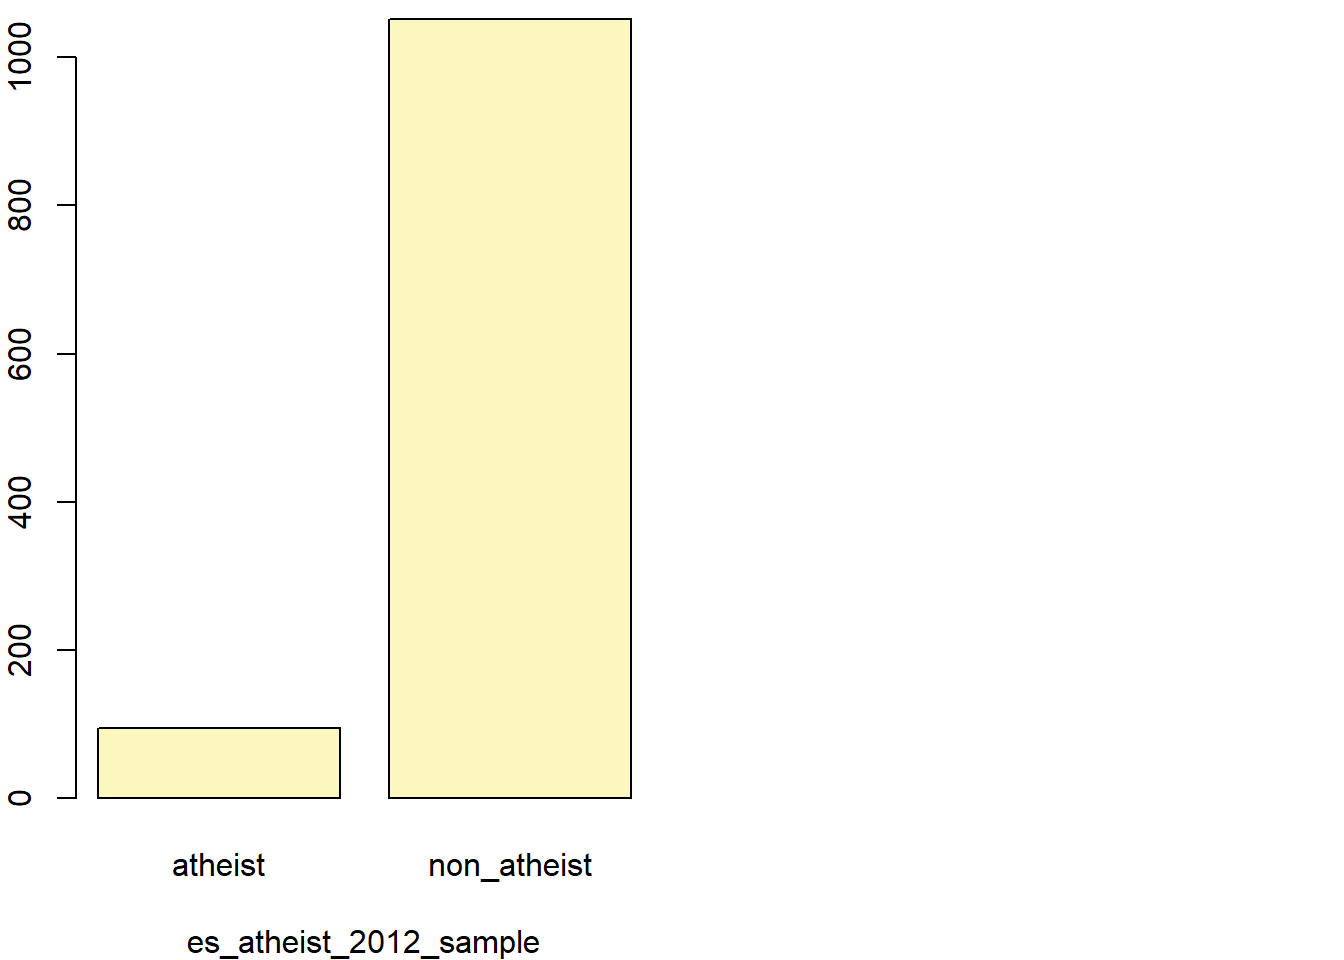
\includegraphics{Santosh-intro_to_r_files/figure-latex/unnamed-chunk-2-1.pdf}

Finally, in addition to simple mathematical operators like subtraction
and division, you can ask R to make comparisons like greater than,
\texttt{\textgreater{}}, less than, \texttt{\textless{}}, and equality,
\texttt{==}. For example, we can ask if boys outnumber girls in each
year with the expression

\begin{Shaded}
\begin{Highlighting}[]
\NormalTok{arbuthnot}\OperatorTok{$}\NormalTok{boys }\OperatorTok{>}\StringTok{ }\NormalTok{arbuthnot}\OperatorTok{$}\NormalTok{girls}
\end{Highlighting}
\end{Shaded}

\begin{verbatim}
##  [1] TRUE TRUE TRUE TRUE TRUE TRUE TRUE TRUE TRUE TRUE TRUE TRUE TRUE TRUE
## [15] TRUE TRUE TRUE TRUE TRUE TRUE TRUE TRUE TRUE TRUE TRUE TRUE TRUE TRUE
## [29] TRUE TRUE TRUE TRUE TRUE TRUE TRUE TRUE TRUE TRUE TRUE TRUE TRUE TRUE
## [43] TRUE TRUE TRUE TRUE TRUE TRUE TRUE TRUE TRUE TRUE TRUE TRUE TRUE TRUE
## [57] TRUE TRUE TRUE TRUE TRUE TRUE TRUE TRUE TRUE TRUE TRUE TRUE TRUE TRUE
## [71] TRUE TRUE TRUE TRUE TRUE TRUE TRUE TRUE TRUE TRUE TRUE TRUE
\end{verbatim}

This command returns 82 values of either \texttt{TRUE} if that year had
more boys than girls, or \texttt{FALSE} if that year did not (the answer
may surprise you). This output shows a different kind of data than we
have considered so far. In the \texttt{arbuthnot} data frame our values
are numerical (the year, the number of boys and girls). Here, we've
asked R to create \emph{logical} data, data where the values are either
\texttt{TRUE} or \texttt{FALSE}. In general, data analysis will involve
many different kinds of data types, and one reason for using R is that
it is able to represent and compute with many of them.

This seems like a fair bit for your first lab, so let's stop here. To
exit RStudio you can click the \emph{x} in the upper right corner of the
whole window.\\
You will be prompted to save your workspace. If you click \emph{save},
RStudio will save the history of your commands and all the objects in
your workspace so that the next time you launch RStudio, you will see
\texttt{arbuthnot} and you will have access to the commands you typed in
your previous session. For now, click \emph{save}, then start up RStudio
again.

\begin{center}\rule{0.5\linewidth}{\linethickness}\end{center}

\subsection{On Your Own}\label{on-your-own}

In the previous few pages, you recreated some of the displays and
preliminary analysis of Arbuthnot's baptism data. Your assignment
involves repeating these steps, but for present day birth records in the
United States. Load up the present day data with the following command.

\begin{Shaded}
\begin{Highlighting}[]
\KeywordTok{source}\NormalTok{(}\StringTok{"more/present.R"}\NormalTok{)}
\end{Highlighting}
\end{Shaded}

The data are stored in a data frame called \texttt{present}.

\subsubsection{\texorpdfstring{\textbf{Q1. What years are included in
this data set? What are the dimensions of the data frame and what are
the variable or column
names?}}{Q1. What years are included in this data set? What are the dimensions of the data frame and what are the variable or column names?}}\label{q1.-what-years-are-included-in-this-data-set-what-are-the-dimensions-of-the-data-frame-and-what-are-the-variable-or-column-names}

\begin{Shaded}
\begin{Highlighting}[]
\NormalTok{years_data <-}\StringTok{ }\KeywordTok{c}\NormalTok{(present}\OperatorTok{$}\NormalTok{year)}
\NormalTok{years_data}
\end{Highlighting}
\end{Shaded}

\begin{verbatim}
##  [1] 1940 1941 1942 1943 1944 1945 1946 1947 1948 1949 1950 1951 1952 1953
## [15] 1954 1955 1956 1957 1958 1959 1960 1961 1962 1963 1964 1965 1966 1967
## [29] 1968 1969 1970 1971 1972 1973 1974 1975 1976 1977 1978 1979 1980 1981
## [43] 1982 1983 1984 1985 1986 1987 1988 1989 1990 1991 1992 1993 1994 1995
## [57] 1996 1997 1998 1999 2000 2001 2002
\end{verbatim}

\begin{Shaded}
\begin{Highlighting}[]
\KeywordTok{dim}\NormalTok{(present)}
\end{Highlighting}
\end{Shaded}

\begin{verbatim}
## [1] 63  3
\end{verbatim}

\begin{Shaded}
\begin{Highlighting}[]
\KeywordTok{names}\NormalTok{(present)}
\end{Highlighting}
\end{Shaded}

\begin{verbatim}
## [1] "year"  "boys"  "girls"
\end{verbatim}

\subsubsection{\texorpdfstring{\textbf{Q2. How do these counts compare
to Arbuthnot's? Are they on a similar
scale?}}{Q2. How do these counts compare to Arbuthnot's? Are they on a similar scale?}}\label{q2.-how-do-these-counts-compare-to-arbuthnots-are-they-on-a-similar-scale}

We cannot compare between \texttt{Arbuthnot} data and \texttt{Present}
data since the data time period (16th vs 19th century) doesn't match.
However, the count of baptized boys and girls is significantly lower
when compared to the count in Present data.

\subsubsection{\texorpdfstring{\textbf{Q3. Make a plot that displays the
boy-to-girl ratio for every year in the data set. What do you see? Does
Arbuthnot's observation about boys being born in greater proportion than
girls hold up in the U.S.? Include the plot in your
response.}}{Q3. Make a plot that displays the boy-to-girl ratio for every year in the data set. What do you see? Does Arbuthnot's observation about boys being born in greater proportion than girls hold up in the U.S.? Include the plot in your response.}}\label{q3.-make-a-plot-that-displays-the-boy-to-girl-ratio-for-every-year-in-the-data-set.-what-do-you-see-does-arbuthnots-observation-about-boys-being-born-in-greater-proportion-than-girls-hold-up-in-the-u.s.-include-the-plot-in-your-response.}

\textbf{\texttt{Arbuthnot} and \texttt{Present} data set both present an
observation where boys ratio is slightly higher than girls. However,
there is a clear visible downtrend in boys ratio in \texttt{Present}
data}

\begin{Shaded}
\begin{Highlighting}[]
\KeywordTok{plot}\NormalTok{(present}\OperatorTok{$}\NormalTok{year, present}\OperatorTok{$}\NormalTok{boys}\OperatorTok{/}\NormalTok{present}\OperatorTok{$}\NormalTok{girls, }\DataTypeTok{type =} \StringTok{"l"}\NormalTok{, }\DataTypeTok{main  =} \StringTok{"Boys to Girls ratio (Present)"}\NormalTok{, }\DataTypeTok{xlab =} \StringTok{"Years"}\NormalTok{, }\DataTypeTok{ylab =} \StringTok{"Boys/Girls"}\NormalTok{)}
\end{Highlighting}
\end{Shaded}

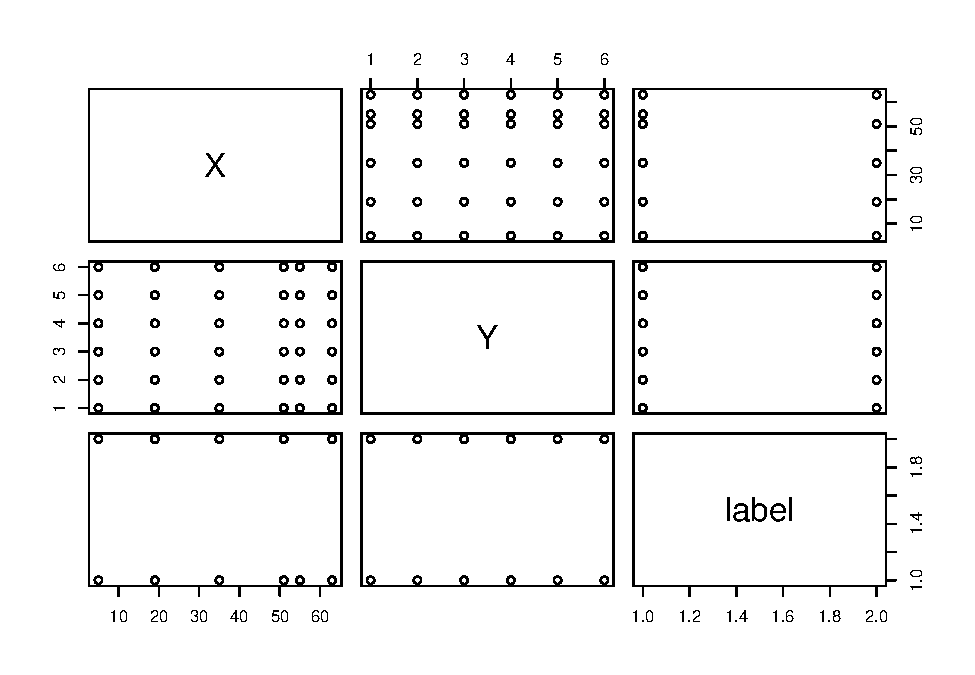
\includegraphics{Santosh-intro_to_r_files/figure-latex/unnamed-chunk-4-1.pdf}

\begin{Shaded}
\begin{Highlighting}[]
\KeywordTok{plot}\NormalTok{(arbuthnot}\OperatorTok{$}\NormalTok{year, arbuthnot}\OperatorTok{$}\NormalTok{boys}\OperatorTok{/}\NormalTok{arbuthnot}\OperatorTok{$}\NormalTok{girls, }\DataTypeTok{type =} \StringTok{"l"}\NormalTok{, }\DataTypeTok{main  =} \StringTok{"Boys to Girls ratio (Arbuthnot)"}\NormalTok{, }\DataTypeTok{xlab =} \StringTok{"Years"}\NormalTok{, }\DataTypeTok{ylab =} \StringTok{"Boys/Girls"}\NormalTok{)}
\end{Highlighting}
\end{Shaded}

\includegraphics{Santosh-intro_to_r_files/figure-latex/unnamed-chunk-4-2.pdf}

\subsubsection{\texorpdfstring{\textbf{Q4. In what year did we see the
most total number of births in the U.S.? You can refer to the help files
or the R reference card
\url{http://cran.r-project.org/doc/contrib/Short-refcard.pdf} to find
helpful
commands.}}{Q4. In what year did we see the most total number of births in the U.S.? You can refer to the help files or the R reference card http://cran.r-project.org/doc/contrib/Short-refcard.pdf to find helpful commands.}}\label{q4.-in-what-year-did-we-see-the-most-total-number-of-births-in-the-u.s.-you-can-refer-to-the-help-files-or-the-r-reference-card-httpcran.r-project.orgdoccontribshort-refcard.pdf-to-find-helpful-commands.}

\begin{Shaded}
\begin{Highlighting}[]
\NormalTok{present}\OperatorTok{$}\NormalTok{total_birth <-}\StringTok{ }\NormalTok{present}\OperatorTok{$}\NormalTok{boys }\OperatorTok{+}\StringTok{ }\NormalTok{present}\OperatorTok{$}\NormalTok{girls}
\NormalTok{max_birth_year <-}\StringTok{ }\NormalTok{present[}\KeywordTok{which.max}\NormalTok{(present}\OperatorTok{$}\NormalTok{total_birth),]}\OperatorTok{$}\NormalTok{year}
\NormalTok{max_birth_year}
\end{Highlighting}
\end{Shaded}

\begin{verbatim}
## [1] 1961
\end{verbatim}

These data come from a report by the Centers for Disease Control
\url{http://www.cdc.gov/nchs/data/nvsr/nvsr53/nvsr53_20.pdf}. Check it
out if you would like to read more about an analysis of sex ratios at
birth in the United States.

That was a short introduction to R and RStudio, but we will provide you
with more functions and a more complete sense of the language as the
course progresses. Feel free to browse around the websites for
\href{http://www.r-project.org}{R} and
\href{http://rstudio.org}{RStudio} if you're interested in learning
more, or find more labs for practice at \url{http://openintro.org}.

\hypertarget{license}{}
This is a product of OpenIntro that is released under a
\href{http://creativecommons.org/licenses/by-sa/3.0}{Creative Commons
Attribution-ShareAlike 3.0 Unported}. This lab was adapted for OpenIntro
by Andrew Bray and Mine Çetinkaya-Rundel from a lab written by Mark
Hansen of UCLA Statistics.


\end{document}
